\appchapter{设计控制方案}
我们的控制设计遵循以下假设:

\begin{enumerate}
  \item 物体的惯性参数$\left( {I,m,{l_{cm}}} \right)$ 是已知的,
    但我们允许扭转摩擦系数 $\mu_{tors}$ 存在不确定性。
    惯性参数可以在旋转任务之前使用力-力矩传感器来测量$^{[23]}$。
    由于转动摩擦系数取决于接触几何形状和压力分布,因此在实际中难以测量。
    这证明在 $\mu_{tors}$ 上使用自适应控制器是正确的。
  \item 已知目标物体的视觉模型,通过视觉系统跟踪目标的位置 $\theta$ 。
  \item 通过触觉传感器测量手指施加的法向力 $f_n$ 。
  \item 该夹持器的方向可以 使物体在重力矩的作用下朝特定方向 旋转,即
    ${\mathop{\rm sgn}} ({\tau _g}) = {\mathop{\rm sgn}} ({\theta _d} - {\theta _0})$
  \item 已知软指变形模型(6)的指数 $\gamma$ 。此参数取决于指尖材质,
    可以使用(6)或(7)进行离线估计。
  \item 当我们进行被动旋转时,物体的位置 $\theta$ 不能超过目标角度 $\theta_d$ 。
    否则,机械手必须旋转抓取器才能再次执行被动旋转,
    或者我们需要通过加速机械手在物体上产生角动量。
  \item 物体最初处于静止状态并处于被抓握稳定的状态 。
\end{enumerate}


根据假设 2和 3我们将控制器分解为两个子控制器,如图 3 所示。
首先,自适应控制器将视觉系统测量的角度 $\theta$ 和
参考模型给定的期望角度 $\theta_m$ 作为输入,
计算一个参考的法向力 $u_{f_n}$ 来控制目标物的运动轨迹。然后, PI 控制器根据该参
考力 $u_{f_n}$ 与触觉测量的法向力 $f_n$ 来调整手指的开合速度,
使测量力与参考法向力之间的误差最小化。

\begin{figure}[!ht]
  \centering
  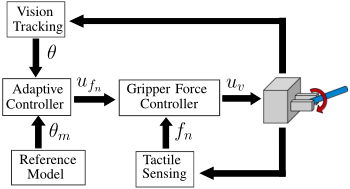
\includegraphics[scale=1]{appendices/pic/4-1}
  \caption*{
    \mtb{图3}我们所建议的旋转控制方案概述}
  \vspace{-0.3cm}
\end{figure}


\appsection{自适应控制器}

我们选择模型参考自适应控制,因为我们的目标是在给定的转动摩擦系数 $\mu_{tors}$
存在误差的情况下正确执行旋转任务,即允许非线性模型(9)中的参数存在不确定性。

自适应控制通过按照参考模型定义的状态轨迹${{\mathop{\rm x}\nolimits} _m}(t) = {\left[ {{\theta _m}(t),{{\dot \theta }_m}(t)} \right]^T}$
驱动系统的状态${\mathop{\rm x}\nolimits} (t) = {\left[ {\theta (t),\dot \theta (t)} \right]^T}$
来执行跟踪控制。
该参考模型由用户自行设计,描述了系统应遵循的理想响应,
满足任务的控制要求和约束条件。在该项目中,角度响应不应超调,
因此,我们将参考模型设计为具有单位直流增益的临界阻尼二阶系统,
其传递函数如下

\stepcounter{appequ}
\vspace{-15pt}
\begin{equation}
  {H_m}(p) = \frac{{{\theta _m}}}{{{\theta _{in}}}} = \frac{{\lambda _0^2}}{{{{\left( {p + {\lambda _0}} \right)}^2}}}
\end{equation}

\noindent 其中,参考输入 $\theta_{in}$ 表示阶跃信号。

为了制定我们的控制器,我们改写了公式(8)中的动力学模型,将法向力作为控制输入 $u_{f_n}$

\stepcounter{appequ}
\vspace{-15pt}
\begin{equation}
  h\ddot {\theta}  + b{\tau _g} = u_{{f_n}}^{1 + \gamma }
\end{equation}

\noindent 式中, $h = 0.5I\mu _{tors}^{ - 1}$和 $b = 0.5\mu _{tors}^{ - 1}$。
然后定义以下跟踪控制误差$s$

\stepcounter{appequ}
\vspace{-15pt}
\begin{equation}
  s = \dot {\tilde \theta}  + \lambda \tilde \theta
\end{equation}

\noindent 式中 $\tilde \theta  = \theta  - {\theta _m}$ 和$\dot {\tilde \theta}  = \dot {\theta}  - {\dot {\theta _m}}$
分别表示角位置和速度误差, $\lambda$ 为常数。

然后我们可以定义标准的自适应控制方程$^{24]}$

\stepcounter{appequ}
\vspace{-15pt}
\begin{equation}
  u_{{f_n}}^{1 + \gamma } = \hat h{\ddot {\theta _r}} - {k_s}s + \hat b{\tau _g}
\end{equation}


该控制方程由速度误差和前向加速度项 $\hat h{\ddot {\theta _r}}$ 、
跟踪误差项 $k_s s$ 和非线性的重力补偿项 $\hat b{\tau _g}$ 构成,
参考角加速度 ${\ddot {\theta _r}}$ 由
${\ddot {\theta _r}} = {\ddot {\theta _m}} - \lambda \dot {\tilde \theta}$
给定,$k_s$ 为正跟踪控制增益。$\hat h$ 和$\hat b$ 分别为 $h$ 和 $b$ 的自适应估计值。

\stepcounter{appequ}
\vspace{-15pt}
\begin{equation}
  \dot {\hat h} =  - {\alpha _h}s{\ddot {\theta _r}}
\end{equation}

\stepcounter{appequ}
\vspace{-15pt}
\begin{equation}
  \dot {\hat b} =  - {\alpha _b}s{\tau _g}
\end{equation}

\noindent 其中 $\alpha_h$ , $\alpha_b$ 为正适应增益。
需要注意的是,除非满足持续激励条件,
否则在线估计值(14a),(14b)不能保证对应参数收敛到真值。
我们不认为这是一个主要的限制,因为我们的工作范围是执行旋转任务,
而不是准确估计摩擦参数。
事实上,该控制方案保证了跟踪误差的收敛性,这意味着被控物体能旋转到指定的角度。


\appsection{夹爪力控}
我们用 PI 控制器来调节法向力 $f_n$

\stepcounter{appequ}
\vspace{-15pt}
\begin{equation}
  {u_v} = {k_p}{\tilde f_n} + {k_i}\int_0^t {{{\tilde f}_n}dt}
\end{equation}

\noindent 式中, $u_v$ 是夹持器的速度设定点, $k_p$ 、 $k_i$ 为控制器激励,
且 ${\tilde f_n} = {f_n} - {u_{{f_n}}}$ 是测量的法向力 $f_n$ 和
根据自适应控制方程式(13)计算的法向力设定值 $u_{f_n}$ 之间的误差。
调节控制器使 ${f_n} \to {u_{{f_n}}}$。

